\documentclass[12pt]{article}
\usepackage[margin=2cm]{geometry}
\usepackage{titling}
\usepackage{graphicx}
\usepackage{float}
\usepackage[hidelinks]{hyperref}
\usepackage[italian]{babel}
\usepackage{subcaption}

\setlength\parindent{0pt}
\setlength{\parskip}{1em}
\setlength{\droptitle}{-2cm}

\title{Istruzioni d'uso TableFootballPlus}
\author{Università della Svizzera Italiana}
\date{Versione \today}


\begin{document}
\maketitle
\tableofcontents
\newpage

\section{Setup}

	\subsection{Montaggio}

		//TODO
		
		
	\subsection{Preparazione all'uso}
	
		.//TODO
		
		

\section{Utilizzo}	
	
	\begin{figure}[H]
        \begin{subfigure}{0.5\textwidth}
                %\includegraphics[width=0.9\textwidth]{img/btn1.jpg}
                \caption*{I pulsanti dal lato dei bianchi}
        \end{subfigure}
        \begin{subfigure}{0.5\textwidth}
                %\includegraphics[width=0.9\textwidth]{img/btn2.jpg}
                \caption*{I pulsanti dal lato dei gialli}
         \end{subfigure}
	\end{figure}
	
	
	
\section{Circuito}

	//TODO
	
	\begin{figure}[H]
                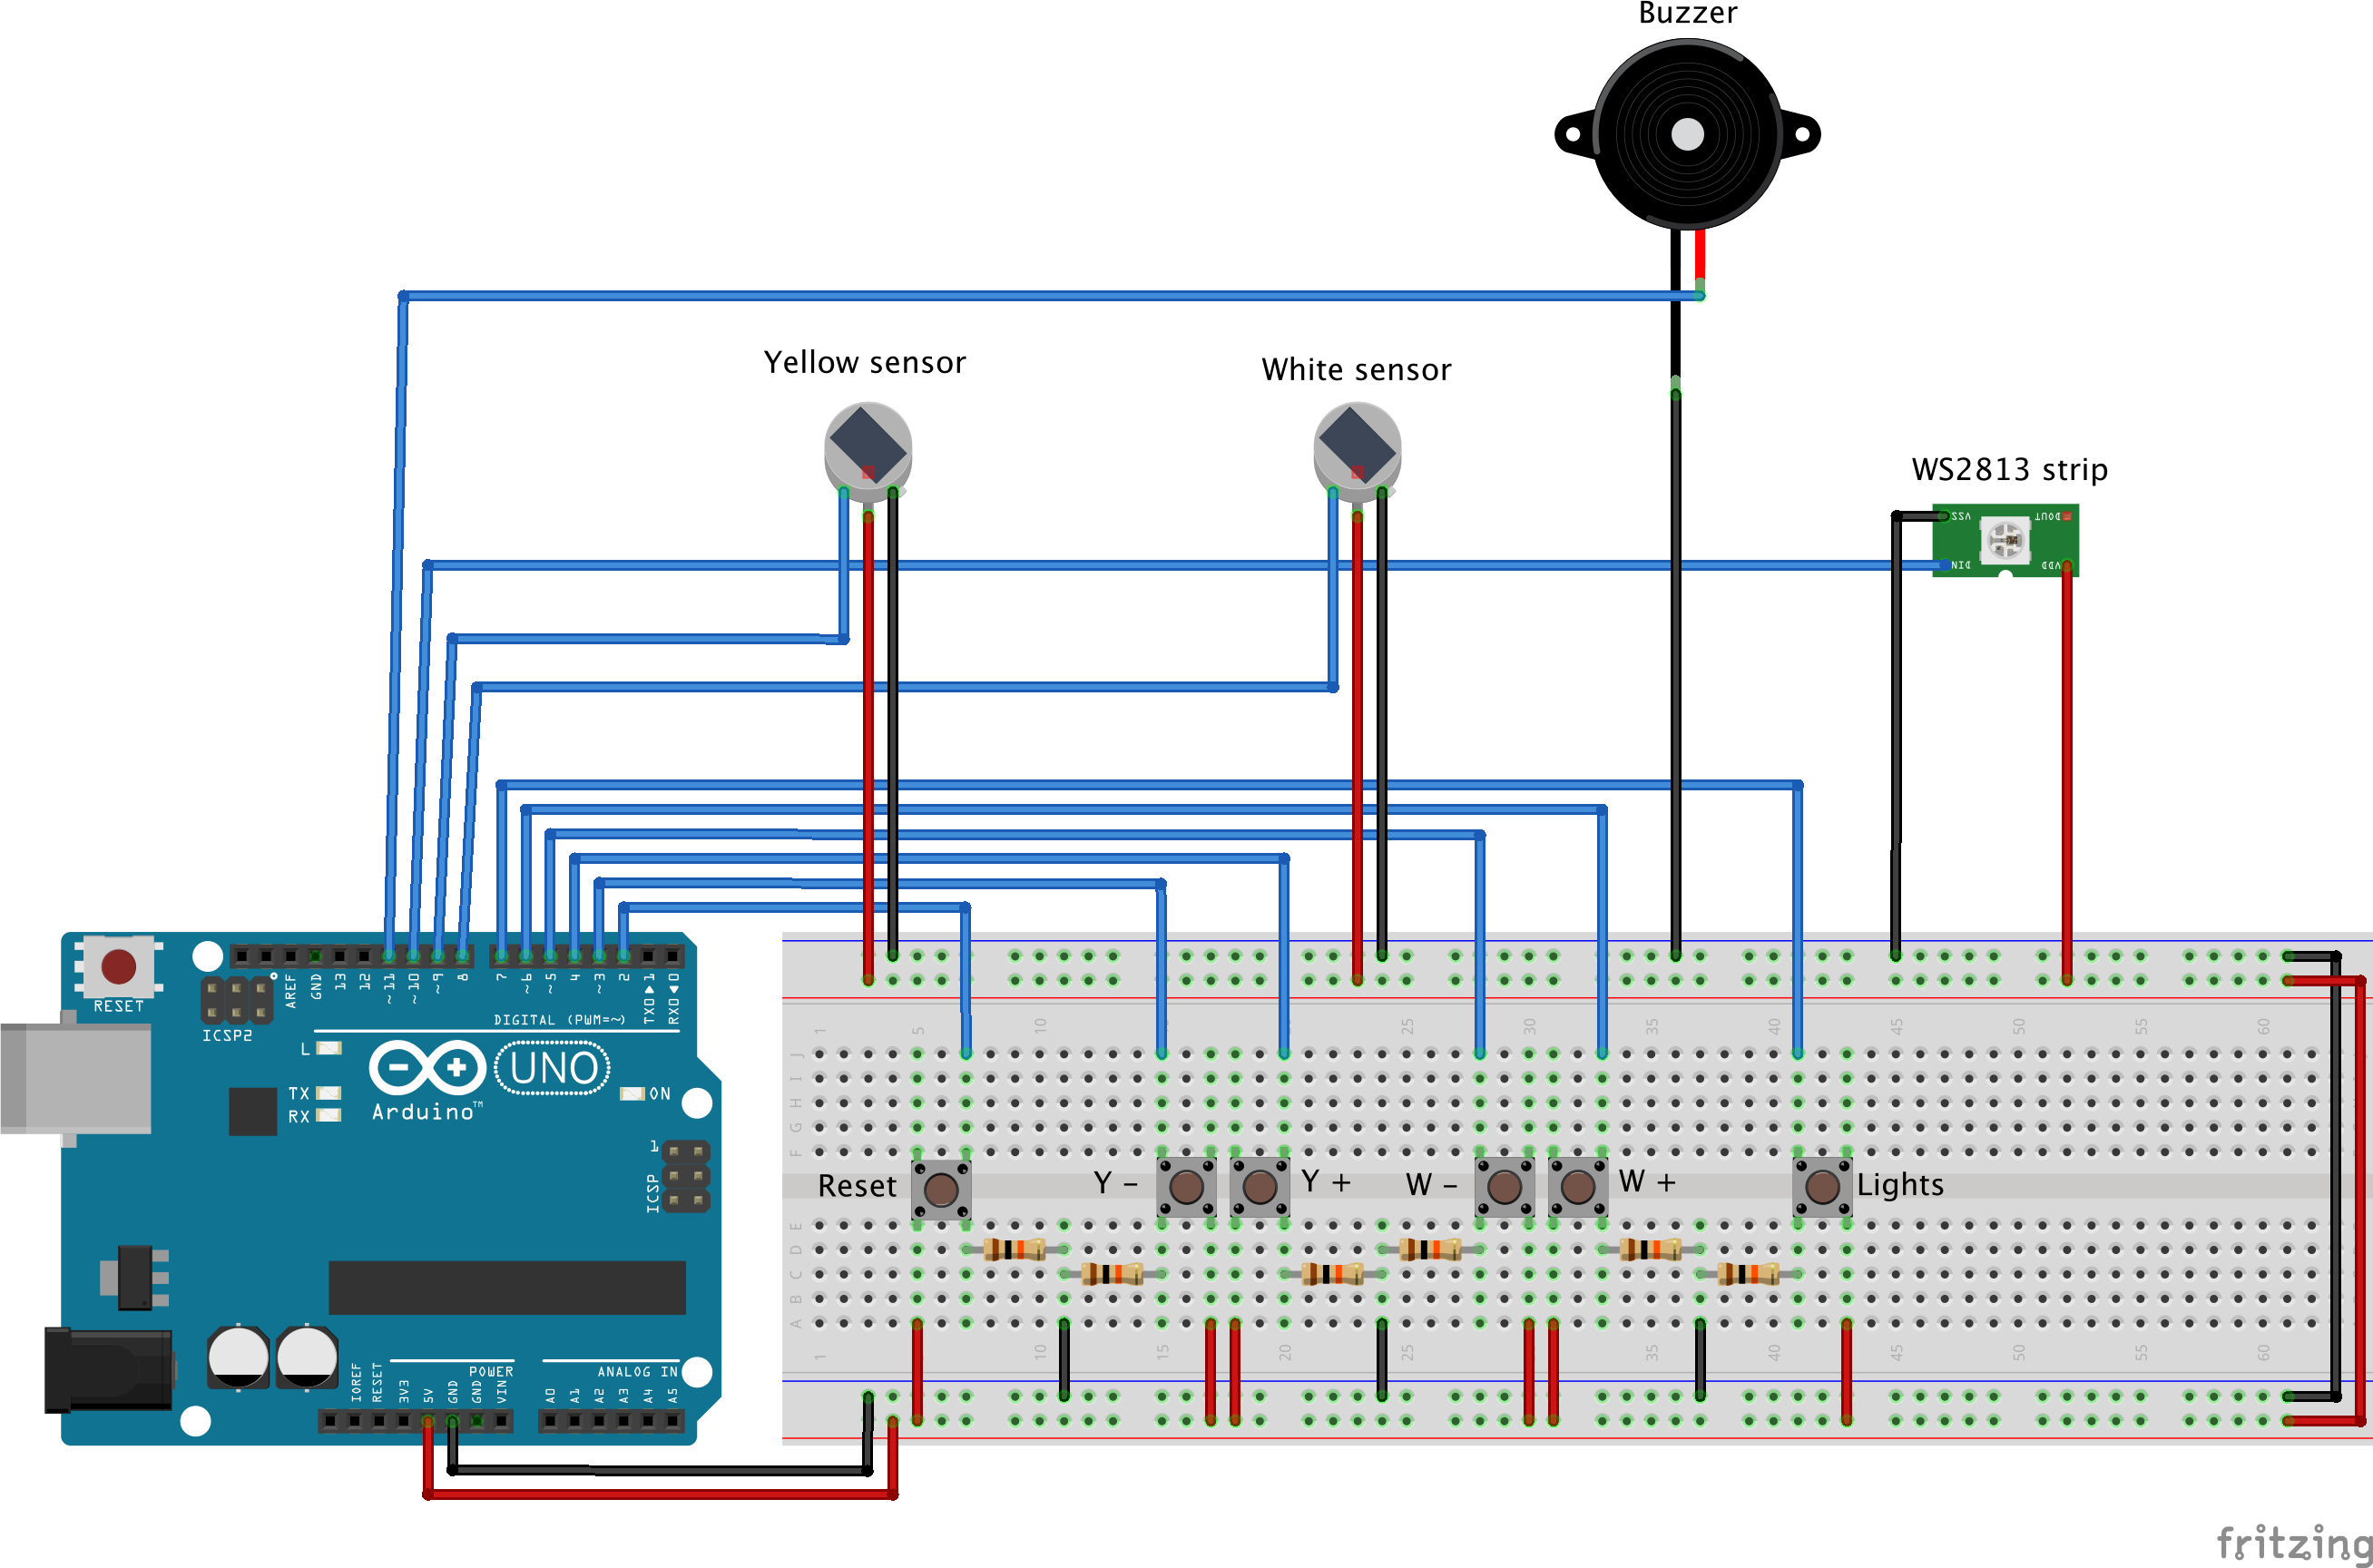
\includegraphics[width=\textwidth]{img/circuit.png}
        \end{figure}
	


\section{Codice}

	//TODO
	\url{https://github.com/USI-Showroom/TableFootballPlus}

\end{document}
